%%%%%%%%%%%%%%%%%%%%%%%%%%%%%%%%%%%%%%%%%%%%%%%%%%%%%%%%%%%%%%%%%%%%%%%%%%%

\documentclass{standalone}

\usepackage{amsmath}
\usepackage{mathptmx}
\usepackage{pgfplots}
\usetikzlibrary{external}
\tikzexternalize{aluminium-error}
\pgfplotsset{compat=1.16}

%% IEEE uses Times Roman font, so we'll default to Times.
%% These three commands make up the entire times.sty package.
\renewcommand{\rmdefault}{ptm}
\renewcommand{\ttdefault}{pcr}
\normalfont\selectfont

\begin{document}

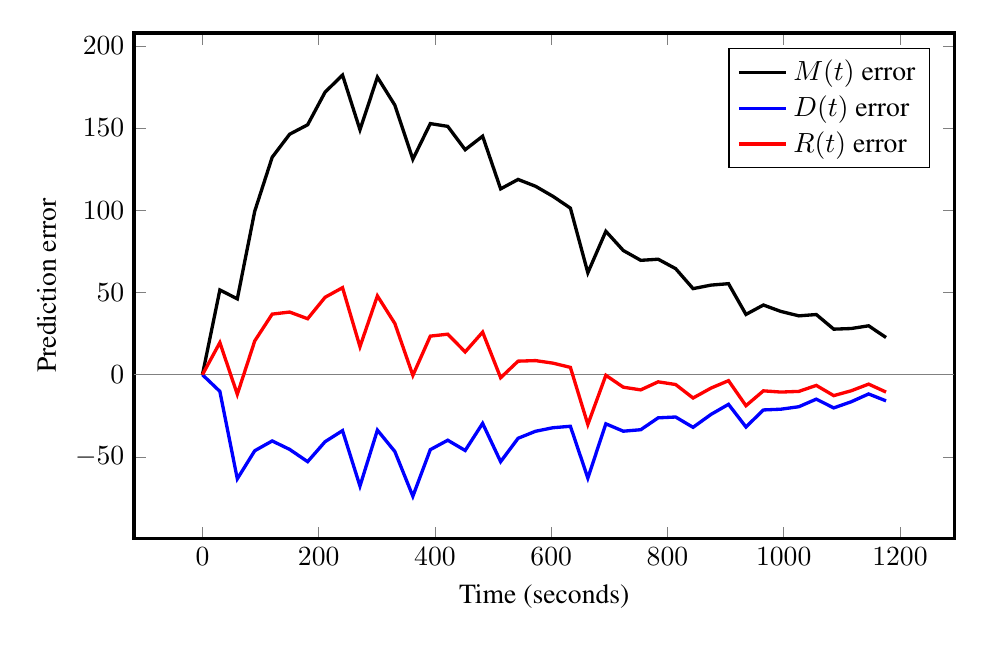
\begin{tikzpicture}
\tikzset{%%
  every mark/.append style={scale=1.0},%%
  scale=1.0%%
}
\pgfplotsset{%%
  every axis/.append style={font=\normalsize}%%
}
%%
\begin{axis}[%%
  axis line style=very thick,%%
  enlargelimits=true,%%
  height=8cm,%%
  legend cell align=left,%%
  legend pos=north east,%%
  plotStyle/.style={very thick,mark=none},%%
  width=12cm,%%
  %% x axis
  xlabel={\normalsize Time~(seconds)},%%
  xtick={0,200,400,600,800,1000,1200},%%
  xticklabels={$0$,$200$,$400$,$600$,$800$,$1000$,$1200$},%%
  %% y axis
  ylabel={\normalsize Prediction error},%%
  scaled y ticks=false,%%
  y tick label style=/pgf/number format/fixed%%
]
%%
%%
%% Horizontal line through origin.
\draw[gray,thin] ({rel axis cs:0,0}|-{axis cs:0,0}) -- ({rel axis cs:1,0}|-{axis cs:1,0});
%%
%%
%% The errors from the function M(t).
\addplot[plotStyle,black] coordinates {
  (0, 0)
  (30, 51.553553)
  (60, 46.1363438570429)
  (90, 99.4555718852954)
  (120, 132.239713931963)
  (150, 146.236978160241)
  (181, 151.995175891345)
  (211, 171.823730454497)
  (241, 182.208158786099)
  (271, 148.962728095272)
  (301, 180.915202607317)
  (331, 163.905862749046)
  (362, 131.013539038131)
  (392, 152.703172169769)
  (422, 151.014077351364)
  (452, 136.828438364318)
  (482, 145.037000576821)
  (513, 113.009646899172)
  (543, 118.748455868656)
  (573, 114.596280329137)
  (603, 108.472529233899)
  (633, 101.302468007001)
  (663, 62.0167929593998)
  (694, 87.2158007730592)
  (724, 75.5351417466817)
  (754, 69.5579665310921)
  (784, 70.2331536612442)
  (814, 64.5132966178352)
  (844, 52.3544338659137)
  (875, 54.5030208737394)
  (905, 55.3622708498656)
  (935, 36.6677629894767)
  (965, 42.3870693207945)
  (995, 38.4901183803216)
  (1026, 35.8034754793119)
  (1056, 36.6029547197058)
  (1086, 27.7076816031795)
  (1116, 28.095474088758)
  (1146, 29.7457620822021)
  (1176, 22.6394702974505)
};
\addlegendentry{$M(t)$ error}
%%
%%
%% The errors from the function D(t).
\addplot[plotStyle,blue] coordinates {
  (0, 0)
  (30, -10.1344439084614)
  (60, -63.2866100321988)
  (90, -46.2171066392607)
  (120, -40.2627381781323)
  (150, -45.4015669090994)
  (181, -52.8630628054216)
  (211, -40.7156839228503)
  (241, -33.9896445624152)
  (271, -67.6948893332084)
  (301, -33.686317889978)
  (331, -46.6875871670834)
  (362, -73.8801707649148)
  (392, -45.5574308035501)
  (422, -39.8279449226129)
  (452, -46.0611926043023)
  (482, -29.5699314780223)
  (513, -52.8647831724983)
  (543, -38.6403455314351)
  (573, -34.3757352441318)
  (603, -32.2306378210552)
  (633, -31.3402241285453)
  (663, -62.8189138346963)
  (694, -29.8535134368972)
  (724, -34.3322942031416)
  (754, -33.4305368217779)
  (784, -26.2066608528401)
  (814, -25.7101173862733)
  (844, -31.9827658659919)
  (875, -24.092947830042)
  (905, -17.9997882901551)
  (935, -31.7674121670323)
  (965, -21.4171917503984)
  (995, -20.967218292925)
  (1026, -19.4470283559494)
  (1056, -14.8389561591472)
  (1086, -20.1707158820307)
  (1116, -16.4515444245064)
  (1146, -11.6892606535397)
  (1176, -15.8904830971262)
};
\addlegendentry{$D(t)$ error}
%%
%%
%% The errors from the function R(t).
\addplot[plotStyle,red] coordinates {
  (0, 0)
  (30, 19.5438237302718)
  (60, -11.8879976669507)
  (90, 20.555529587205)
  (120, 36.8571000456745)
  (150, 38.1160133000544)
  (181, 34.046374362916)
  (211, 47.0896034072436)
  (241, 52.9419789213062)
  (271, 17.0522695009571)
  (301, 47.9324266920447)
  (331, 31.1503428682476)
  (362, -0.390631475444223)
  (392, 23.4807657875974)
  (422, 24.6593329445143)
  (452, 13.8806188066786)
  (482, 25.9104839675955)
  (513, -1.84529590157173)
  (543, 8.24793270324352)
  (573, 8.5913114019918)
  (603, 7.04154616193576)
  (633, 4.47176752200961)
  (663, -30.2303520156148)
  (694, -0.349889333151019)
  (724, -7.58237180394071)
  (754, -9.21509947880166)
  (784, -4.31681712988502)
  (814, -5.94838990298437)
  (844, -14.1637064918366)
  (875, -8.09953145627005)
  (905, -3.60979520115876)
  (935, -18.8323288430901)
  (965, -9.80011242741437)
  (995, -10.5423457784342)
  (1026, -10.1331353708264)
  (1056, -6.49333275585657)
  (1086, -12.6976223266445)
  (1116, -9.76387446495192)
  (1146, -5.70791122323865)
  (1176, -10.5437411071639)
};
\addlegendentry{$R(t)$ error}
\end{axis}
\end{tikzpicture}

\end{document}
